%%%%%%%%%%%%%%%%%%%%%%%%%%%%%%%%%%%%%%%%%
% Wenneker Assignment
% LaTeX Template
% Version 2.0 (12/1/2019)
%
% This template originates from:
% http://www.LaTeXTemplates.com
%
% Authors:
% Vel (vel@LaTeXTemplates.com)
% Frits Wenneker
%
% License:
% CC BY-NC-SA 3.0 (http://creativecommons.org/licenses/by-nc-sa/3.0/)
%
%%%%%%%%%%%%%%%%%%%%%%%%%%%%%%%%%%%%%%%%%

%----------------------------------------------------------------------------------------
%	PACKAGES AND OTHER DOCUMENT CONFIGURATIONS
%----------------------------------------------------------------------------------------

\documentclass[11pt]{scrartcl} % Font size
\usepackage{comment}
\usepackage{color}
%%%%%%%%%%%%%%%%%%%%%%%%%%%%%%%%%%%%%%%%%
% Wenneker Assignment
% Structure Specification File
% Version 2.0 (12/1/2019)
%
% This template originates from:
% http://www.LaTeXTemplates.com
%
% Authors:
% Vel (vel@LaTeXTemplates.com)
% Frits Wenneker
%
% License:
% CC BY-NC-SA 3.0 (http://creativecommons.org/licenses/by-nc-sa/3.0/)
% 
%%%%%%%%%%%%%%%%%%%%%%%%%%%%%%%%%%%%%%%%%

%----------------------------------------------------------------------------------------
%	PACKAGES AND OTHER DOCUMENT CONFIGURATIONS
%----------------------------------------------------------------------------------------

\usepackage{amsmath, amsfonts, amsthm} % Math packages
\usepackage{tabto}
\usepackage{listings} % Code listings, with syntax highlighting
\usepackage{tabu}
\usepackage{array}
\usepackage[english]{babel} % English language hyphenation
\usepackage{hyperref}

\usepackage{graphicx} % Required for inserting images
\graphicspath{{Figures/}{./}} % Specifies where to look for included images (trailing slash required)

\usepackage{booktabs} % Required for better horizontal rules in tables

\numberwithin{equation}{section} % Number equations within sections (i.e. 1.1, 1.2, 2.1, 2.2 instead of 1, 2, 3, 4)
\numberwithin{figure}{section} % Number figures within sections (i.e. 1.1, 1.2, 2.1, 2.2 instead of 1, 2, 3, 4)
\numberwithin{table}{section} % Number tables within sections (i.e. 1.1, 1.2, 2.1, 2.2 instead of 1, 2, 3, 4)

\setlength\parindent{0pt} % Removes all indentation from paragraphs

\usepackage{enumitem} % Required for list customisation
\setlist{noitemsep} % No spacing between list items

%----------------------------------------------------------------------------------------
%	DOCUMENT MARGINS
%----------------------------------------------------------------------------------------

\usepackage{geometry} % Required for adjusting page dimensions and margins

\geometry{
	paper=a4paper, % Paper size, change to letterpaper for US letter size
	top=2.5cm, % Top margin
	bottom=3cm, % Bottom margin
	left=3cm, % Left margin
	right=3cm, % Right margin
	headheight=0.75cm, % Header height
	footskip=1.5cm, % Space from the bottom margin to the baseline of the footer
	headsep=0.75cm, % Space from the top margin to the baseline of the header
	%showframe, % Uncomment to show how the type block is set on the page
}

%----------------------------------------------------------------------------------------
%	FONTS
%----------------------------------------------------------------------------------------

\usepackage[utf8]{inputenc} % Required for inputting international characters
\usepackage[T1]{fontenc} % Use 8-bit encoding

\usepackage{fourier} % Use the Adobe Utopia font for the document

%----------------------------------------------------------------------------------------
%	SECTION TITLES
%----------------------------------------------------------------------------------------

\usepackage{sectsty} % Allows customising section commands

\sectionfont{\vspace{6pt}\centering\normalfont\scshape} % \section{} styling
\subsectionfont{\normalfont\bfseries} % \subsection{} styling
\subsubsectionfont{\normalfont\itshape} % \subsubsection{} styling
\paragraphfont{\normalfont\scshape} % \paragraph{} styling

%----------------------------------------------------------------------------------------
%	HEADERS AND FOOTERS
%----------------------------------------------------------------------------------------

\usepackage{scrlayer-scrpage} % Required for customising headers and footers

\ohead*{} % Right header
\ihead*{} % Left header
\chead*{} % Centre header

\ofoot*{} % Right footer
\ifoot*{} % Left footer
\cfoot*{\pagemark} % Centre footer
 % Include the file specifying the document structure and custom commands
\usepackage{graphicx}
\usepackage{subcaption}



%Code retrieved from: https://www.overleaf.com/project/5c52d66b6343590b46b4fd03


%----------------------------------------------------------------------------------------
%	TITLE SECTION
%----------------------------------------------------------------------------------------

\title{
	\normalfont\normalsize
	\textsc{Old Dominion University}\\ % Your university, school and/or department name(s)
	\vspace{25pt} % Whitespace
	\rule{\linewidth}{0.5pt}\\ % Thin top horizontal rule
	\vspace{20pt} % Whitespace
	{\huge Assignment 3}\\ % The assignment title
	\vspace{12pt} % Whitespace
	\rule{\linewidth}{2pt}\\ % Thick bottom horizontal rule
	\vspace{12pt} % Whitespace
}

\author{\LARGE David Bayard} % Your name

\date{\normalsize\today} % Today's date (\today) or a custom date

\begin{document}

\definecolor{codegreen}{rgb}{0,0.6,0}
\definecolor{codegray}{rgb}{0.5,0.5,0.5}
\definecolor{codepurple}{rgb}{0.58,0,0.82}
\definecolor{backcolour}{rgb}{0.95,0.95,0.92}
\lstdefinestyle{pythonStyle}{
  backgroundcolor=\color{backcolour},
  commentstyle=\color{codegreen},
  keywordstyle=\color{magenta},
  numberstyle=\tiny\color{codegray},
  stringstyle=\color{codepurple},
  basicstyle=\footnotesize,
  breakatwhitespace=false,
  breaklines=true,
  captionpos=b,
  keepspaces=true,
  numbers=left,
  numbersep=5pt,
  showspaces=false,
  showstringspaces=false,
  showtabs=false,
  tabsize=2
}

\lstset{style=pythonStyle}


\maketitle % Print the title

\pagebreak
\section*{Question 1.}



%------------------------------------------------

\subsection*{Download the 1000 URIs from assignment 2.  "curl", "wget", or
"lynx" are all good candidate programs to use.  We want just the
raw HTML, not the images, stylesheets, etc.}
\bigskip\bigskip


\LARGE Solution:
\newline \newline\small

\tabto{2.0cm} The requests library was used to download the URIs, sending GET requests to each of the URIs and creating a response object from the response. This was repeated for each URI in the list of existing URIs from assignment 2. 

\begin{lstlisting}[language = Python, caption=Download HTML]
   try:
      response = requests.get(uri, allow_redirects=True, timeout=30)

    except Exception as e:
      print('Error: ', str(e))
\end{lstlisting} \bigskip 

\tabto{2.0cm} After downloading the HTML, a hashing function was used to create distinct file names for each URI. The returned hash code and URI were then appended to the ``Records.txt'' file. After creating each file, the .text() method of the response object is used to retrieve the HTML and write it to the new file.

\begin{lstlisting}[language = Python, caption=Make Hashcode]
   with open('tempFile.txt', 'rb') as afile:
        buf = afile.read()
        hasher.update(buf)

    fileName = hasher.hexdigest() + '.html'

    #Write to the specified file (with hash code)
    writeComplete = open(fileName, 'w')

    writeComplete.write(response.text)
\end{lstlisting} \bigskip 

\tabto{2.0cm} ``python-boilerpipe'' was used to extract the HTML from each file. In order to use this library, a virtual environment was created, and the source code was installed in this environment. There were difficulties when installing ``python-boilerpipe'', but this was solved by specifying the Python version to use (3.6) when installing. 

\begin{lstlisting}[language = Python, caption=Extract Text]
with open(a['FileName'] , 'r') as read:
    html = read.read()

  #Extract html from file
  extractor = Extractor(extractor='ArticleExtractor', html=html)
  extractedText = extractor.getText()
\end{lstlisting} \bigskip 

\tabto{2.0cm} The code above is responsible for extracting the majority of the HTML from each hashed document, resulting in new files that contain only the text from the HTML files.

\pagebreak

\section*{Question 2}


\subsection*{Choose a query term (e.g., "shadow") that is not a stop word
(see week 5 slides) and not HTML markup from step 1 (e.g., "http")
that matches at least 10 documents (hint: use "grep" on the processed
files).  If the term is present in more than 10 documents, choose
any 10 from your list.}

%------------------------------------------------
\bigskip\bigskip
\LARGE Solution: \newline\newline\small

\tabto{2.0cm} The query term used was ``Congress''. This query term is relevant within the context of the downloaded documents, and it was expected to have been found in multiple documents. With the query term selected, a search was conducted on each of the document files containing extracted text, using grep as the searching tool.


\begin{lstlisting}[language = Python, caption=Query Term Search]
process = subprocess.Popen(['grep', '-rwn', arg, completeName], stdout=subprocess.PIPE)
    stdout, stderr = process.communicate()
    if len(stdout) != 0:
      num_words = 0
\end{lstlisting} \bigskip 

\tabto{2.0cm} In the above code, there is a list ``stdout'', which contains all of the information retrieved from grep search. Moreover, the if condition filters out any documents that did not match the query term.
\newline

\tabto{2.0cm} Two very important segments of code are listed below. This code is responsible for counting the number of words that each document contains, as well as the number of times the query term appears in the document. This information is then stored in a file for later use. 
\newline

\begin{lstlisting}[language = Python, caption=Word Count and Count for Query Term]
with open(completeName, 'r') as readFile:
        for line in readFile:
          words = line.split()

          ## Keeps track of number of words in file ##
          num_words += len(words)
      
      with open(completeName) as toCount:

        ## Code from Joshua on slack, Counts occurrance of query term in document##
        wordcount = Counter(toCount.read().split()) 
        wordOuccurance = wordcount['Congress']

        if(wordOuccurance != 0): 
          fileCounter += 1
\end{lstlisting}

\pagebreak
\begin{center} \large The following equations listed below were used to calculate the TFIDF, TF, and IDF: \end{center}
 \small

$$ TF = \frac {Occurrances \ of \ Query \ Term} {Total \ Word \ Count} $$
\newline
$$ IDF = \frac {Total \ Number \ of \ Documents} {Documents \ Containing \ Querty \  Term} $$
\newline
$$ TFIDF =  {TF * IDF} $$

\begin{center} \large With regards to normalization for question 3, the following equation was used: \end{center}
$$ Normalized \ Score = \frac {x - x_{min}} {x_{max} - x_{min} }$$
\small \newline

\tabto{2.0cm} All values were rounded to four significant figures (after the decimal) because most of the values for the TF, IDF, and TFIDF were smaller than those of the assignment example. \newline \newline 
\tabto{2.0cm} Moreover, a logarithmic function was not required for the IDF because the total number of documents was used as the corpus, instead of using a search engine. All of the results for the TF, IDF, and TFIDF calculations are stored in the ``CalculationRecords2.txt'' file for future reference. 
\newline

\tabto{2.0cm} In order to calculate the TF, IDF, and TFIDF, the snippet of code supplied below was used. This code takes the data from the ``MatchedFormatted.json'' file and runs it through the formulas supplied above. In this case, the corpus is 1130, and the query term was found in 375 files, found in "fileOccurrance.txt". The TF, IDF, and TFIDF, are then rounded to four significant figures, and are written to a dictionary for later use.

\begin{lstlisting}[language = Python, caption= Calculations]
if(checkURI in collectionURI):
      ## Word Count (Frequency) / Number of words found in document
      TF = entry["WordCount"] / entry["NumberWords"]
      roundedTF = round(TF,4)

      ## Had a total of 1130 documents, Query Term was found in 375 documents out of 1130
      IDF = 1130/375
      roundedIDF = round(IDF,4)
      
      TF_IDF = TF * IDF
      roundedTF_IDF = round(TF_IDF, 4)

      calcData["TFIDF"] = roundedTF_IDF
      calcData["TF"] = roundedTF
      calcData["IDF"] = roundedIDF
      calcData["URI"] = entry["URI"]

      collectionCalc.append(calcData)
\end{lstlisting}

\pagebreak
\tabto{2.0cm} The URIs in the table below were shortened to fit within the coulumn of the table. The full URI and data is provided in the ``CalculationRecords2.txt'' file. 
\newline \newline 
% Code Taken From: https://www.overleaf.com/learn/latex/Tables
\begin{center}
\begin{LARGE} Calculate TF, IDF, and TFIDF  \end{LARGE} \newline \newline
\begin{tabular}{ |p{1cm}||p{1cm}|p{1cm}|p{6cm}|  }
 \hline
 \multicolumn{4}{|c|}{Calculation Records Using Query Term ``Congress''} \\
 \hline
 TFIDF & TF & IDF & URI\\
 \hline
0.0339   & 0.0113   &3.0133&   https://www.numbersusa.com/ \\
0.0324 & 0.0108  & 3.0133   &https://www.facebook.com/ \\
0.0261 & 0.0086 & 3.0133&  https://in.reuters.com/ \\
0.0222 & 0.0074 & 3.0133& https://www.reuters.com/\\
0.0209&   0.0069  & 3.0133&http://www.msn.com/\\
0.0160& 0.0053  & 3.0133   &https://www.cnn.com\\
0.0155& 0.0051  & 3.0133&https://dailywn.com/\\
0.0143& 0.0047  & 3.0133&https://www.upi.com/\\
0.0135& 0.0045  & 3.0133&https://www.vox.com/\\
0.0126& 0.0042  & 3.0133&https://whyy.org/\\
0.0105& 0.0035  & 3.0133&https://www.cnbc.com/\\
0.0099& 0.0033  & 3.0133&https://www.theguardian.com/\\
0.0088& 0.0029  & 3.0133&https://www.nbcnews.com/\\
0.0074& 0.0025  & 3.0133&https://www.nytimes.com/\\
0.0071& 0.0024  & 3.0133&https://newspunch.com/\\
0.0060& 0.0020  & 3.0133&https://apnews.com/\\
0.0034& 0.0011  & 3.0133&https://fullmagazine.us/\\
 \hline
\end{tabular}
\end{center}
\bigskip
\tabto{2.0cm} As an example, the picture below provides an graphical view of what is occurring behind the scenes. This is only a segment of the program though, displaying where each occasion of the Query Term is located, and how many times it occurs.

\begin{figure}[h!]
\begin{subfigure}[b]{1.1\linewidth }
    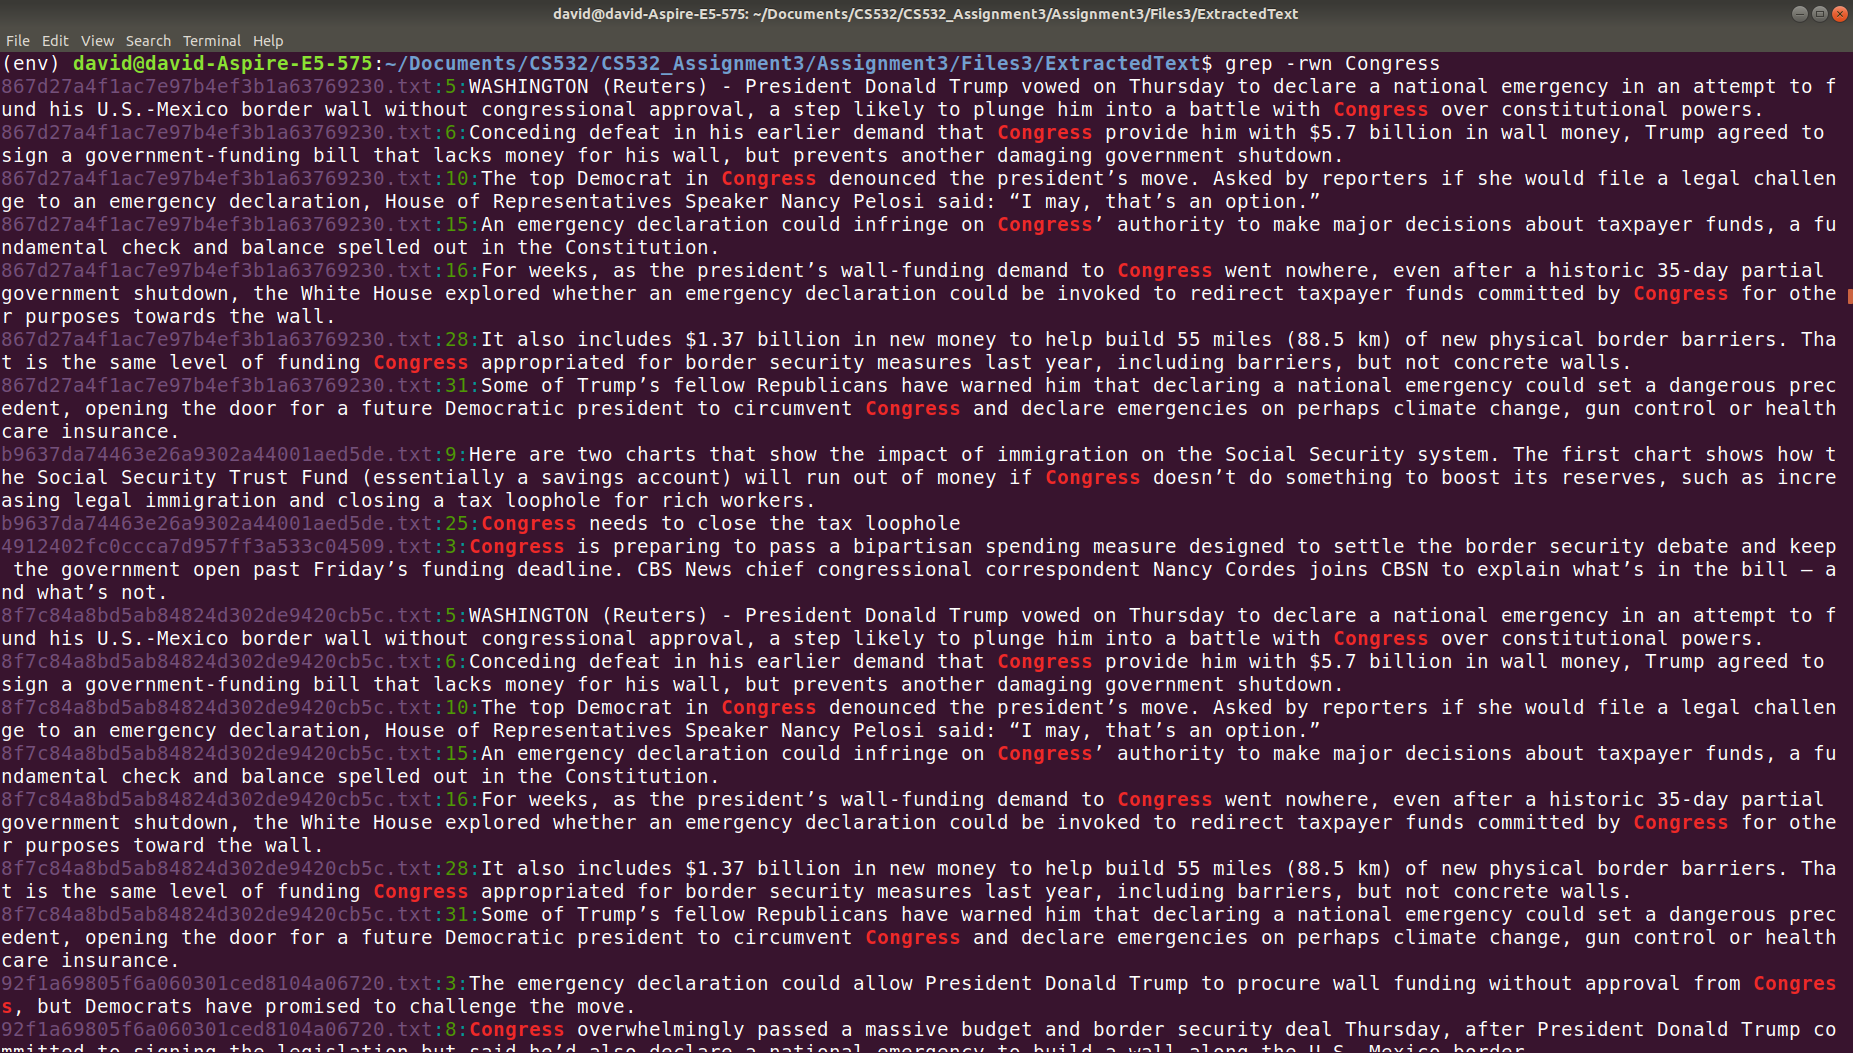
\includegraphics[width=\linewidth]{Proofgrep.png}
    \caption{grep behind the scene}
\end{subfigure}
\end{figure}


\pagebreak
\section*{Question 3} \bigskip

\subsection*{Now rank the same 10 URIs from question 2 but this time 
by their PageRank.  Use any of the free PR estimaters on the web.}

\tabto{2.0cm} The PR estimater used for this assignment was 
\url{http://www.prchecker.info/check_page_rank.php}. There were a few issues that occurred while using the PR estimator, which resulted in less accurate results.
\newline

\tabto{2.0cm} One issue associated with the PR estimator is that it only ranks a page based off of the home page of each URI. This resulted in a less specific PR, as it was not based off of the correct page. Another issue was that several of the chosen URIs had a page rank of zero. These URIs were mentioned in the ``NoRanks.txt'' file, and were not added to the list of normalized ranks in the ``PageRanks.txt'' file.
\newline


\tabto{2.0cm} There was no real code involved with retreiving the page ranks, because of the anti-bot captchas. Instead, the URIs were manually run through the PR estimator. 
A table of each of the page ranks is listed below, displaying the pages that did not have a rank of zero.
\newline

\begin{center}
\begin{LARGE} \tabto{1cm}Page Ranks for 10 URI \end{LARGE} \newline \newline
\begin{tabular}{ |p{1cm}||p{6cm}|  }
 \hline
 \multicolumn{2}{|c|}{Page Ranks} \\
 \hline
 Page Rank & URI\\
 \hline
1.0& https://www.cnn.com/ \\
1.0& https://www.facebook.com/ \\
0.9& https://www.reuters.com/ \\
0.9& https://in.reuters.com/\\
0.9& http://www.msn.com/ \\
0.8& https://www.theguardian.com/ \\
0.8& https://www.upi.com/ \\
0.7& https://www.vox.com/ \\
0.7& https://whyy.org/ \\
0.7& https://www.numbersusa.com/ \\
 \hline
\end{tabular}
\end{center}
\bigskip
\tabto{2.0cm} The Page Rank results seem to be inaccurate, and do not produce a correlation between the page rank and the TF, IDF, and TFIDF scores. For example, https://www.numbersusa.com/ ranks lowest on the Page Rank table, but scores highest on the TFIDF value. \newline \newline
\tabto{2.0cm} Moreover, https://www.facebook.com/ ranks second on both table, contradicting any possible correlation from the previous statement. This hints towards the idea that the page rank website is producing false results, and not ranking pages correctly. This is even more evident by the fact that https://www.nbcnews.com/ did not have a page rank. 
\pagebreak
\section*{Question 4. Extra Credit}
%------------------------------------------------

\subsection*{Compute the Kendall TauB ``b'' score for both lists. Report both the
Tau value and the ``p'' value.}
\bigskip\bigskip


\LARGE Solution:
\newline \newline\small

\tabto{2.0cm} Python scipy provides a function called scipy.stats.kendalltau for this exact purpose. This function was implemented, providing the list of page ranks against the list of TFIDFs, TFs, and IDFs, as shown below. 

\begin{lstlisting}[language = Python, caption=Word Count and Count for Query Term]
  ## Calculate Kendall Tau_b Score TFIDF ##
  tauTFIDF, p_valueTFIDF = sp.stats.kendalltau(normalizedRanks, collectionTFIDF)
\end{lstlisting}

\begin{center}
\begin{LARGE} \tabto{1cm}Tau Calculations \end{LARGE} \newline \newline
\begin{tabular}{ |p{3cm}||p{2cm}|p{2cm}|  }
 \hline
 \multicolumn{3}{|c|}{Correlation} \\
 \hline
 Comparison & Tau & P Value\\
 \hline
TFIDF VS Page Rank & 0.25 &  0.19 \\
 \hline
\end{tabular}
\end{center}
\tabto{2.0cm} As seen in the table above, the Tau b score indicates that there is a minor association between the page ranks and the TFIDF. This is evident by a Tau b score, of .25, indicating that there is an association, but that it is insignificant. 


\end{document}
